\documentclass[11pt]{article}
%Gummi|065|=)
\title{\textbf{Welcome to Gummi 0.6.6}}
\author{Alexander van der Meij\\
		Wei-Ning Huang\\
		Dion Timmermann}
\date{}
\usepackage{graphicx}

\graphicspath{{img/}}

\begin{document}

\maketitle

\section{WSTĘP}

\section{OPIS}

<schemat>

Powyższy rysunek to schemat projektu.
Widać na nim wszystkie stworzone moduły.

Nasz projekt ma strukturę gwiazdzistą, gdyż każdy moduł połączony jest z modułem głównym MASTER.

\subsection{vga\_init}

Moduł vga\_init oblicza timingi, które wymagane są przez standard VGA.
Jego wyjściem jest pozycja aktualnego piksela zapisana jako 20 bitowy wektor.
Moduł ten jako wejście przyjmuje 3 bitowy numer koloru, który ma wyświetlić na pikselu.
Dodatkowo połączony jest z zewnętrznymi pinami Spartana.

Wewnątrz znajdują się dwa liczniki modulo liczące w górę.
Pierwszy z nich odlicza pozycję w poziomie w sygnale HPOS i kiedy osiąga wartość maksymalną, aktywuje impuls VGA\_HS.
Drugi licznik zwiększa pozycję w pionie w sygnale VPOS, kiedy licznik HPOS osiąga wartość maksymalną i odpowiada za przeniesienie aktualnego piksela na początek ekranu aktywując VGA\_VS.

Sygnał wyjściowy POS jest konkatenacją 10-bitowych wektorów HPOS i VPOS. 
Kierowany jest do modułu MASTER.

Kolory ustawiane są poprzez sygnały wyjściowe VGA\_R, VGA\_G, VGA\_B.
Pobierane są z 3-bitowego wektora VGA\_COLOR jeśli aktualna pozycja piksela mieści się w widzialnym zakresie monitora.
W przeciwnym wypadku ustawiany jest kolor czarny "000".

\subsection{ROM}

Pamięci ROM są kluczowymi elementami projektu. Występują dwie instancje pamięci tego typu, które są bitmapami o rozmiarze 100x75 zapisanymi jako monochromatyczne bity.
Pierwsza z nich, MAZE, to zapis struktury labiryntu.
Druga to plansza końcowowa z napisem "CONGRATULATION".




\section{IMPLEMENTACJA}

\subsection{PODRĘCZNIK UŻYTKOWNIKA}

Poniższy podręcznik użytkownika ma na celu krótkie wprowadzenie do obsługi gry, bez zagłębiania się w szczegóły implementacyjne.

Celem gry jest przejście labiryntu kwadratem przy pomocy drązka sterowego w jak najkrótszym czasie. Za dotknięcie ściany naliczana jest kara czasowa w postaci wielokrotnie przyspieszonego liczenia czasu.

\begin{figure}
\centering
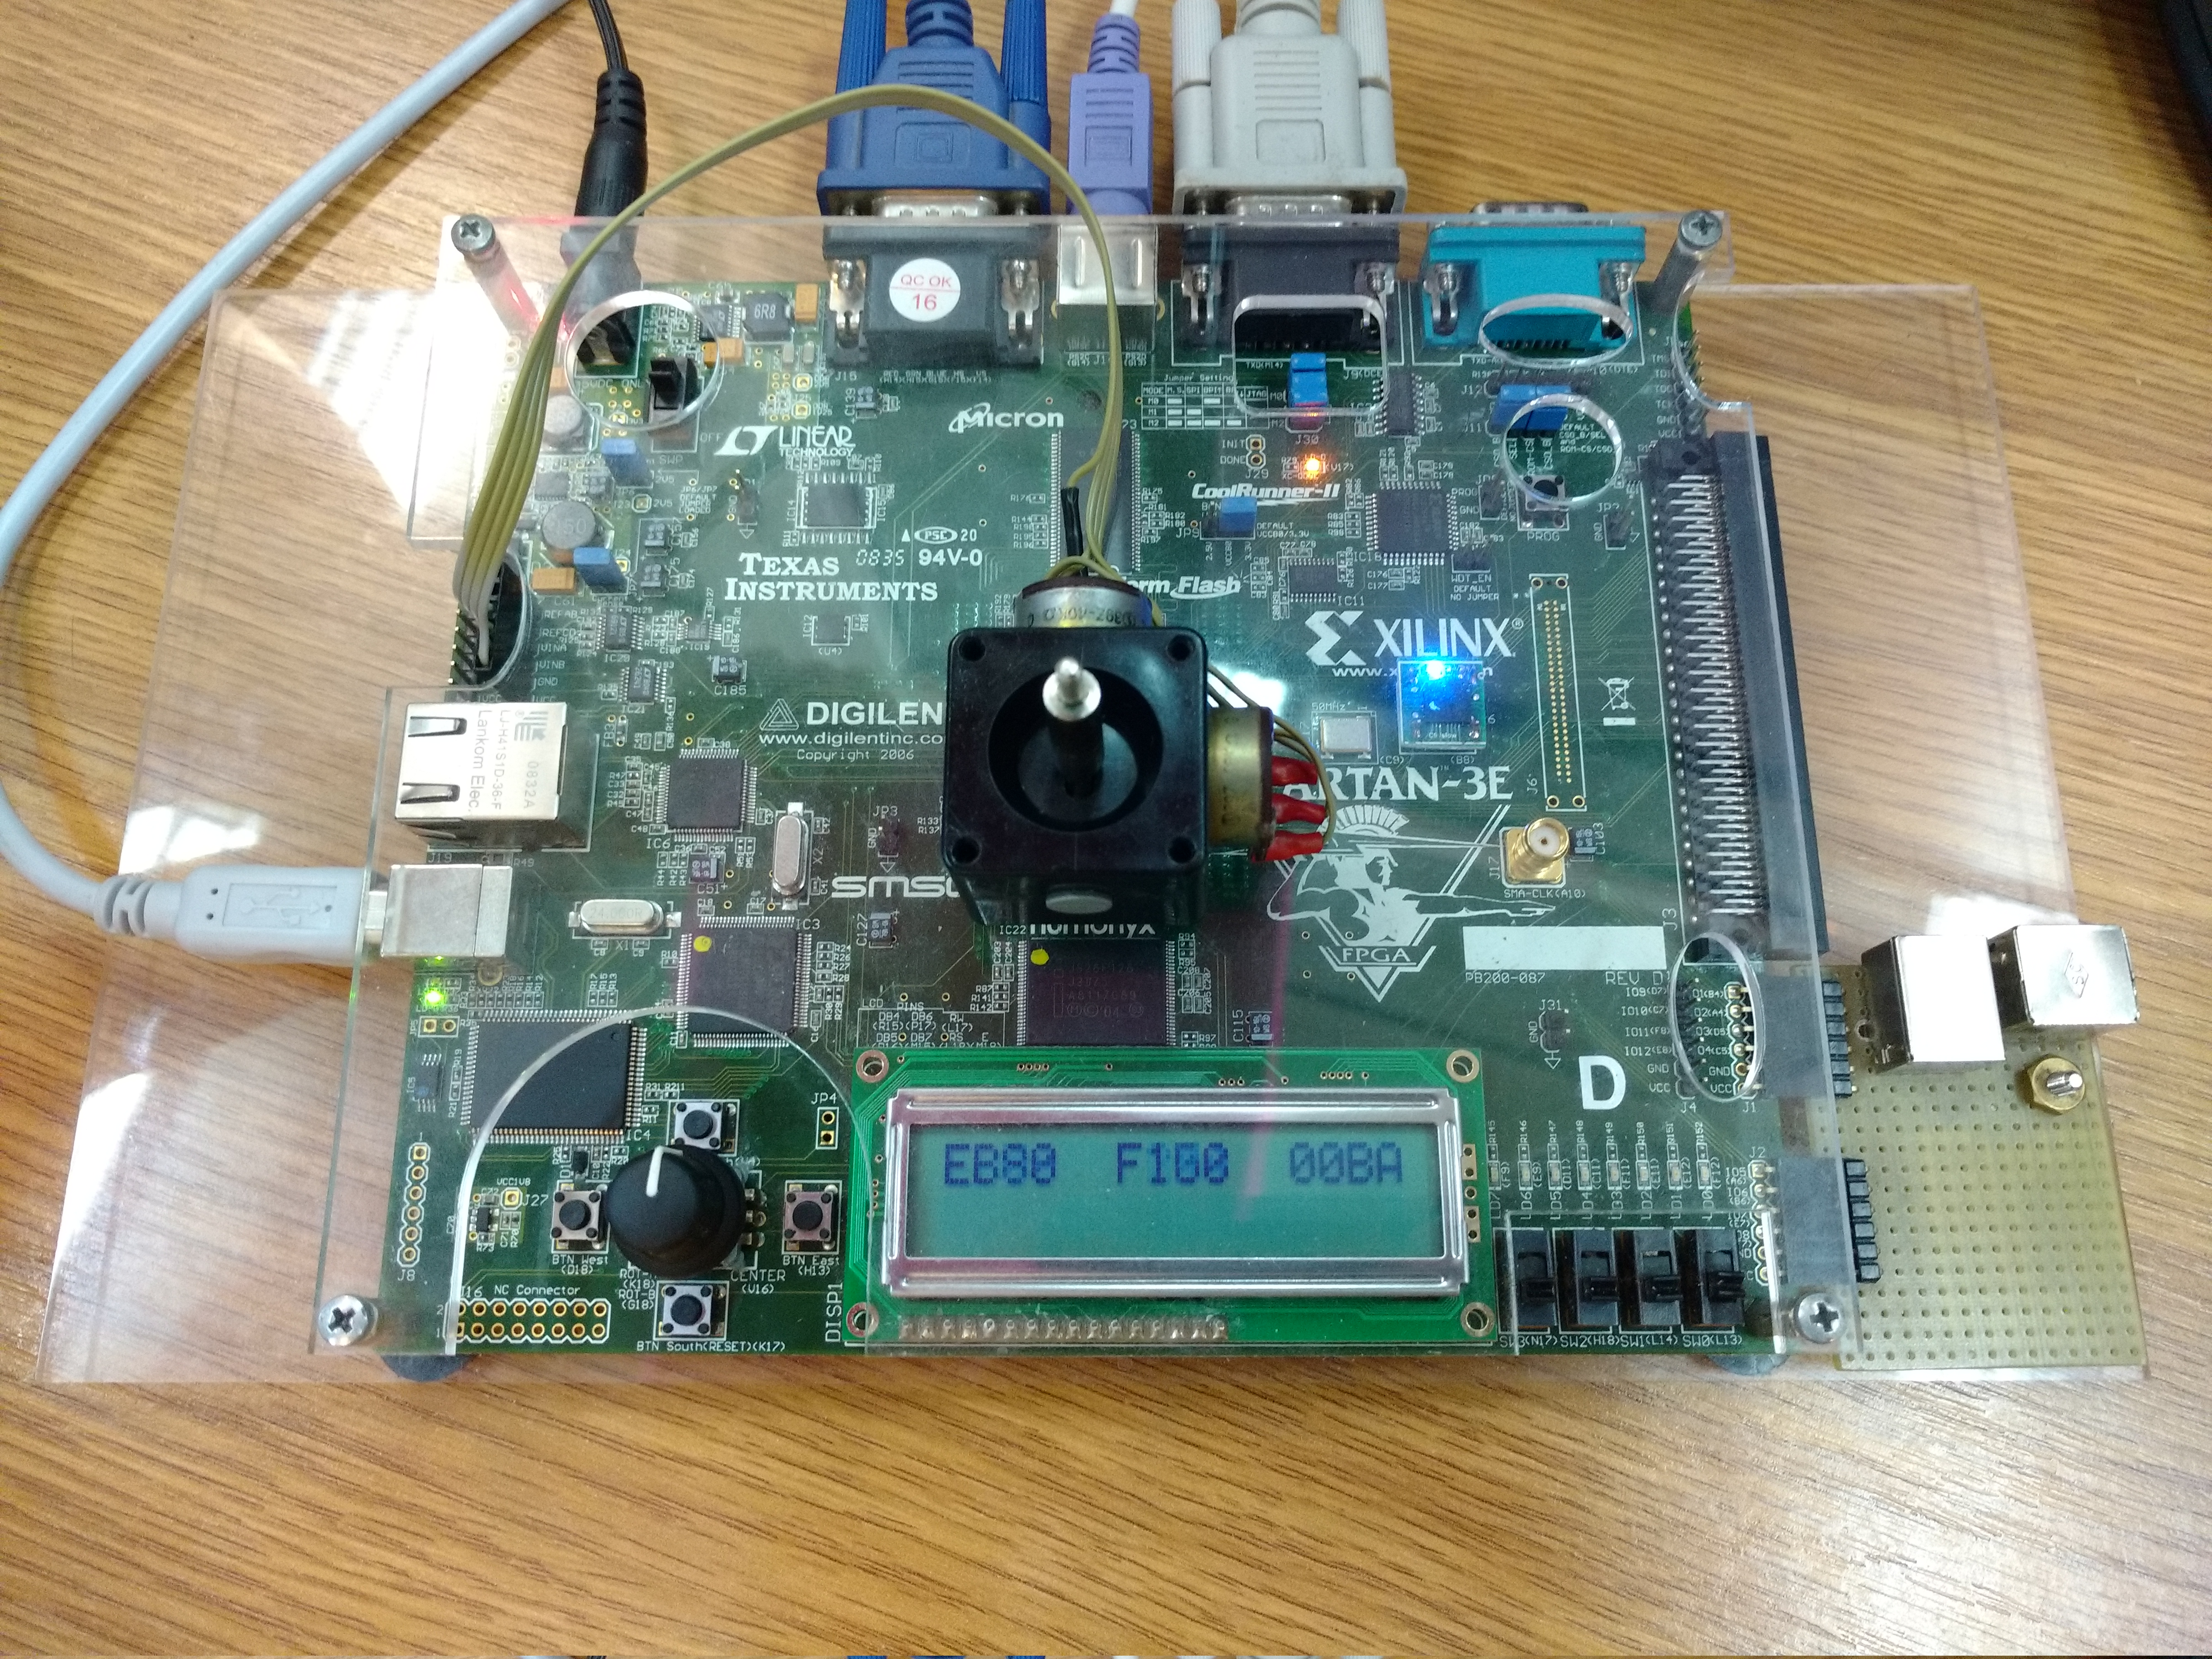
\includegraphics[scale=.05]{plytka}
\caption{Płytka z potrzebnym sprzętem}
\end{figure}

A - wyjście podłączenia monitora przez port VGA \\
B - wejście analogowe do podłączenie drążka sterowego \\
C - analogowy drążek sterowy \\
D - wyświetlacz LCD \\
E - przycisk resetu \\

Jak widać na zdjęciu wtyczka od drążka sterowego musi być podłączona do pinów po prawej stronie i zwrócona widocznymi blaszkami na zewnątrz.

Przed rozpoczęciem gry należy drążek ustawić możliwie w pozycji pionowej.
Oprócz tego należy zwrócić uwagę na to, by osie drążka odpowiadały układowi współrzędnych, gdzie wartości osi X rosną w prawo, a osi Y w górę.
Ma to na celu poprawne odzwierciedlenie ruchów gracza w grze. 
%

Po podłączeniu potrzebnego osprzętu i zaprogramowaniu płytki gra rozpoczyna się. 

Kwadrat w kolorze fuksji, którym poruszamy za pomocą drążka sterowego znajduje się lewym, dolnym rogu.
Gracz poprzez manewrowanie drążkiem sterowym kontroluje ruch kwadratu.
Poruszać się można tylko po żółtym polu. Ściany labiryntu reprezentowane są kolorem niebieskim.
Koniec labiryntu znajduje się w lewym, górnym rogu.
Po dojściu tam, pokazuje się grafika końcowa z napisem "CONGRATULATION". %rys. end-screen
Ponadto zatrzymywany jest pomiar czasu, który pokazany jest na wyświetlaczu LCD po prawej stronie w systemie szesnastkowym.
W celu rozpoczęcia nowej rozgrywki należy użyć przycisku RESET.





\section{PODSUMOWANIE}

Po zakończeniu prac można krytycznie ocenić realizację założeń projektu.
Wszystkie z początkowo postawionych celów zostały spełnione w planowanym terminie, dlatego jesteśmy zadowoleni z ogółu wyników prac.
Pewne rozwiązania, które przyjęliśmy na początku okazały się jednak chybione i po wielogodzinnych analizach problemu oraz pomocy prowadzącego, musieliśmy diametralnie je zmienić.
Przykład może stanowić użycie danych typu integer. Choć zachęcające prostotą użycia, sprawiły nie lada problem dla sprzętu. Okazało się, że należy skorzystać z typu signed.

Kolejną trudnością było przejście z architektury jednomodułowej do wielomodułowej.
Zmiana ta spowodowana była nieczytelnością projektu.
Zbyt wiele procesów w jednym module utrudniało analizę przepływu informacji.
Rozwiązaniem tego problemu było wprowadzenie modułu MASTER, który jako moduł główny łączył pozostałe moduły.
W tym przypadku problematyczne było przeniesienie procesów do MASTERa i dostrojenie ich.

Analizując przebieg prac na projektem, dochodzimy do wniosku, że było kilka elementów, które dałoby się poprawić.
Gdybyśmy jeszcze raz realizowali ten projekt, to od razu dzielilibyśmy system na więcej modułów, by uniknąć problemów przy zmianie.
Ponadto logika sterowania kwadratem również mogłaby być osobnym modułem, co odchudziłoby moduł MASTER.

\subsection{KIERUNKI DALSZYCH PRAC}

Po zakończeniu projektu, pomimo pełnej założonej funkcjonalności, możemy określić dalsze kierunki rozwoju gry.
Przede wszystkim można zaimplementować nowe mapy labiryntów, o rosnącym poziomie trudności, by gra była coraz większym wyzwaniem.
Kolejny pomysł to możliwość zmiany kolorów w grze za pomocą przycisków, które znajdują się dookoła potencjometru na płytce Spartan 3E.
Można również rozbudować projekt o kolejne urządzenia peryferyjne, takie, jak głośnik, na którym odtwarzana byłaby muzyczka umilająca grę.
Następny pomysł, to dodanie obsługi kolejnego drążka sterowego, w celu możliwości gry wieloosobowej na jednym monitorze.
W ten sposób element rywalizacji osiągnąłby wyższy poziom.
Ostatnia propozycja to zapisywanie rankingu czasów osiągniętych przez graczy.


\section{SPIS LITERATURY}


\end{document}
